\Chapter{Hardware Implementation}
\label{chap:hardware}
    The pulsed power supply is implemented using three IGBT modules. The other major hardware components required in this setup are inductors, capacitors and DC power source. The current and voltage sensing have been achieved with the shunt resistors and conditioning circuit. The control algorithm has been implemented on a Texas Instruments F28069 Launchpad. This chapter deals with the methodology used to arrive at the capacitor and inductor sizes suitable for pulsed power application. The complete hardware implementation of the converter topology is presented along with the necessary interfacing and sensing circuits.
	figure \ref{fig:block-diag} shows the top level organisation of the complete hardware setup.
    \begin{figure}[h]
        \centering
        \includegraphics[width=0.8\textwidth]{ConvSch}
        \caption{Block Diagram of Hardware Setup}
        \label{fig:block-diag}
    \end{figure}

\section{Sizing of Passive Components}
\subsection{Inductor Selection}
	The purpose of inductor in DC-DC switched power supplies is to maintain the current when the DC link switch is off i.e. to reduce the ripple in output voltage or current depending on the converter. With this criteria, the inductor value should be high, but when a large inductor is used, the rise time of converter is more as it takes more time for the current to rise. Hence, the selection of inductor is trade-off between the current ripple and transient response of the converter. 

	For the single quadrant converter which is used as current source, criteria for selection of inductor value is taken to be the the inductor current ripple. The relation between inductor value and this ripple \cite{book:768263} is 
	\begin{equation}
		\Delta I_L = \dfrac{V_{o1}}{L_1} (1-D) T_s
		\label{eq:ind-1}
	\end{equation}
	where $V_{o1} = I_{\text{ref}} R_L$ is the output voltage of the single quadrant converter, $L_1$ is the value of the inductor, $D$ is the steady state duty cycle of the converter, $\Delta I_L$ is the ripple in in inductor current and $T_s = \dfrac{1}{F_s}$ is the switching period.
	\begin{equation}
		L_1 \geq \dfrac{V_{o1}(V_d-V_{o1})}{\Delta I_L F_s V_d}
		\label{eq:ind-1a}
	\end{equation}
	Based on these calculations, inductor $L_1$ must be grater than 2 mH. 

	For the voltage source, the boundary condition for continuous conduction mode operation governs the choice of inductor. Because the output current need not be controlled here, the ripple criteria is relaxed in favour of ensuring the continuous conduction mode of the current source. This is ensured whenever the following criteria is satisfied \cite{book:768263}
	\begin{equation}
		I_{L_2} \geq \dfrac{DT_s}{2L_2}(V_d-V_{o2})
		\label{eq:ind-2}
	\end{equation}
	If the average inductor current $I_{L_{\text{avg}}}$ becomes less than this boundary value, the converter operates in discontinuous mode. To extend the range of operation of the converter to lower average currents, the inductor is chosen such that continuous conduction mode is ensured at the lowest extreme of the intended range of operation. For satisfactory operation \cite{muhamad2005design} at $\dfrac{1}{5}I_{L_2}$, the condition in inequality \eqref{eq:ind-1} is
	\begin{equation}
		\dfrac{1}{5}I_{L_2} \geq \dfrac{DT_s}{2L_2}(V_d-V_{o2})
		\label{eq:ind-3}
	\end{equation}
	where $I_{L_2} = V_d / R_L$, $D$ is the steady state duty cycle, $T_s = 1 / F_s$ is the switching period, $L_2$ is the inductor value, and $V_d$ and $V_o = V_{\text{ref}}$ are the DC link and converter output voltages respectively. 
	Therefore,
	\begin{equation}
		L_2 \geq 2.5\dfrac{DT_s}{I_{L_2}}(V_d-V_{\text{ref}})
		\label{eq:ind-4}
	\end{equation}
	Based on this relation the inductor for voltage source must be greater than 0.15 mH.

\subsection{Capacitor Selection}
	Capacitor is required in the output stage of two quadrant converter to filter out the output voltage ripple. For a ripple of $\Delta V_{o2}$, the value of capacitor required is given by\cite{book:768263}
	\begin{equation}
		C_2 \geq \dfrac{\Delta I_{L_2}T_s}{8\Delta V_{o2}}
		\label{eq:ind-4a}
	\end{equation}
	The current ripple is given by,
	\begin{equation}
		\Delta I_{L_2} \geq \dfrac{V_{o2}}{L_2}(1-D) T_s
		\label{eq:ind-4b}
	\end{equation}
	Here, $V_{o2} = V_{\text{ref}}$ and $T_s = 1 / F_s$,
	\begin{equation}
		C_2 \geq \dfrac{1 - D}{8 \dfrac{\Delta V_{o2}}{V_{\text{ref}}}L_2 F_s^2}
		\label{eq:ind-5}
	\end{equation}
	The capacitor must be larger than $10 \mu F$.
	
\subsection{Trajectory based selection of L and C}
    The above calculations only provide a desired range of the inductors and capacitors. This treatement is enough for design of standard DC-DC converters. But, in the proposed pulsed power supply, the current source output will act as disturbance to the voltage source once the ignition switch is opened. To withstand these disturbances the value of inductor and capacitor must account for the settling time and stability.
	\begin{figure}[h]
	\begin{subfigure}{\textwidth}
		\begin{subfigure}{0.49\textwidth}
		\centering
			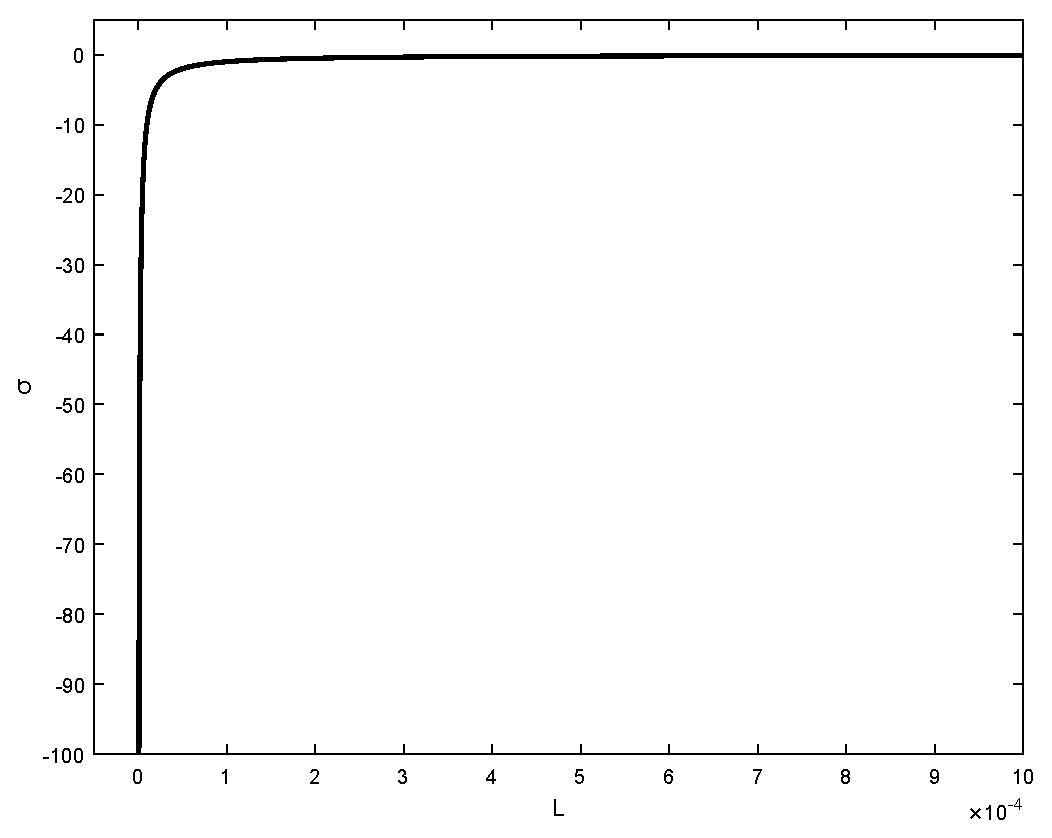
\includegraphics[width=\linewidth]{pd_real_vs_l2}
			\caption{$\sigma$ vs $L_2$}
			\label{fig:pd_real_vs_l2}
		\end{subfigure}
		\begin{subfigure}{0.49\textwidth}
			\centering
			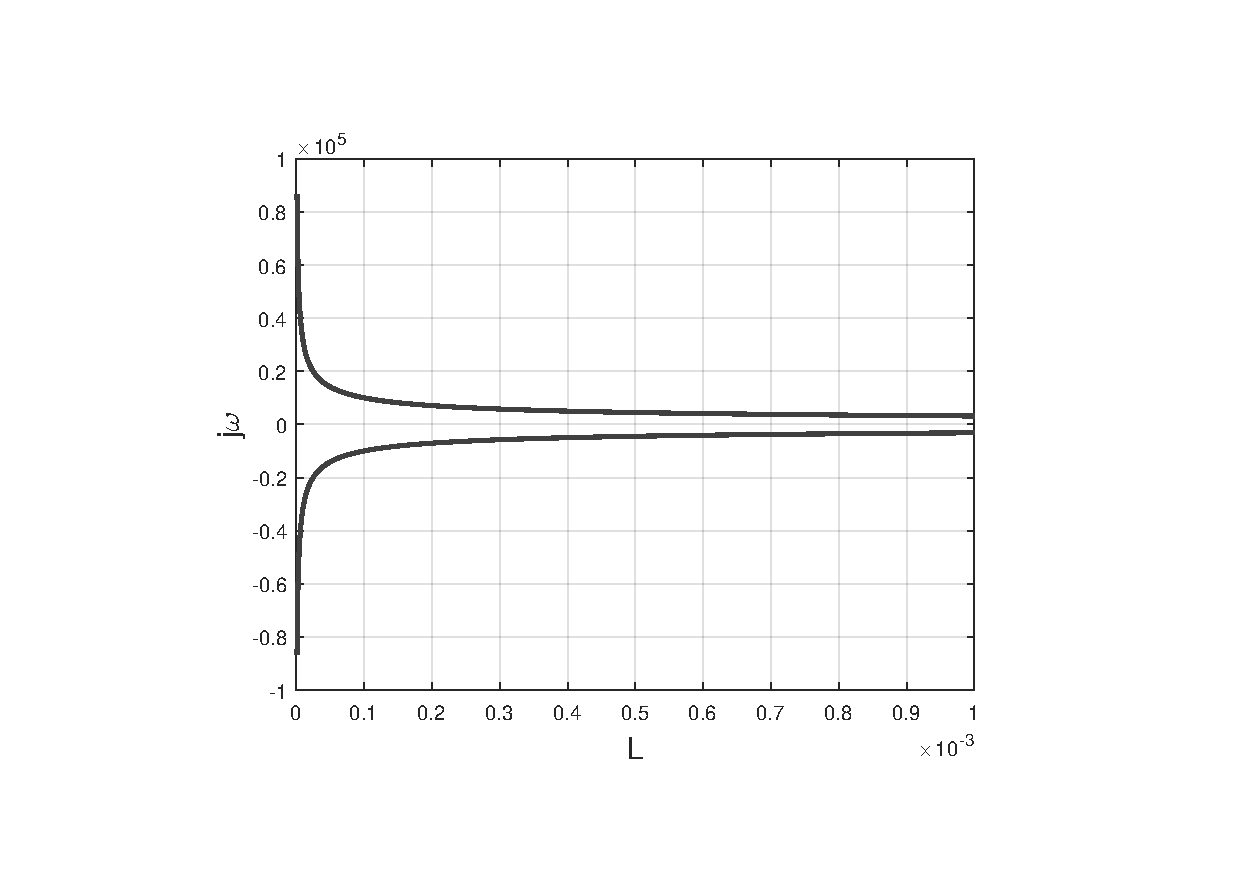
\includegraphics[width=\linewidth]{pd_imag_vs_l2}
			\caption{$j\omega$ vs $L_2$}
			\label{fig:pd_imag_vs_l2}
		\end{subfigure}
	\end{subfigure}
	\begin{subfigure}{\textwidth}
			\begin{subfigure}{0.49\textwidth}
			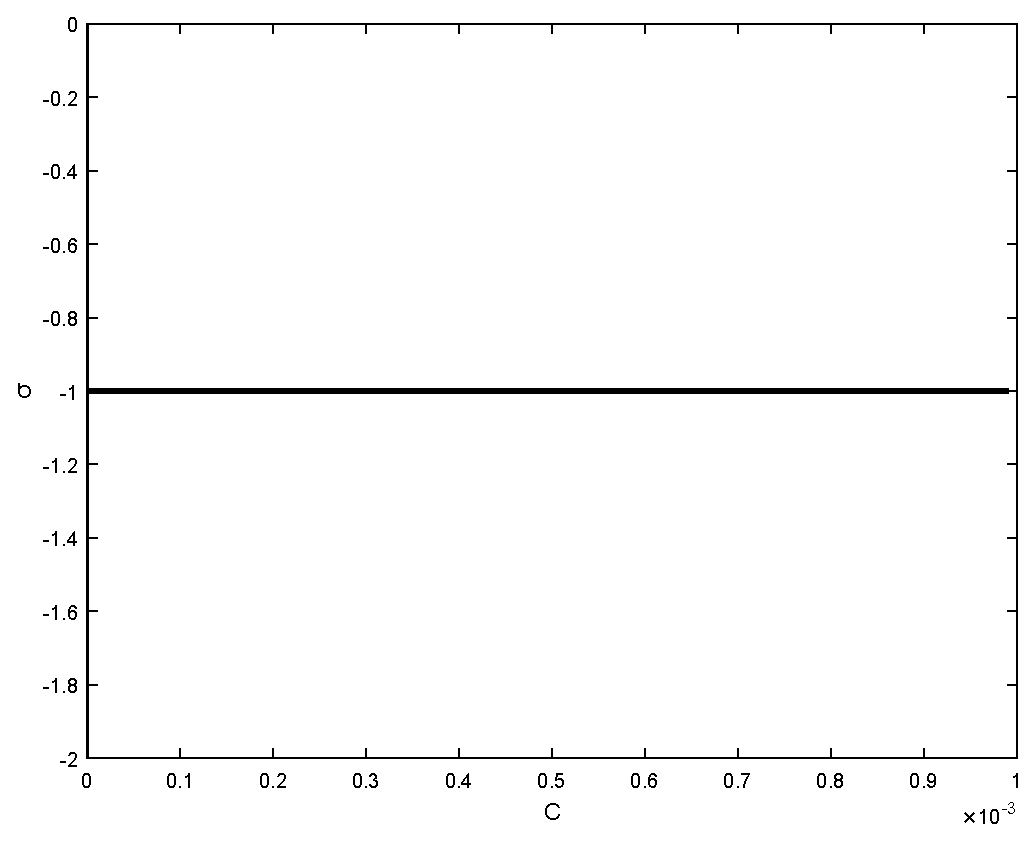
\includegraphics[width=\linewidth]{pd_real_vs_c2}
			\caption{$\sigma$ vs $C_2$}
			\label{fig:pd_real_vs_c2}
		\end{subfigure}
		\begin{subfigure}{0.49\textwidth}
			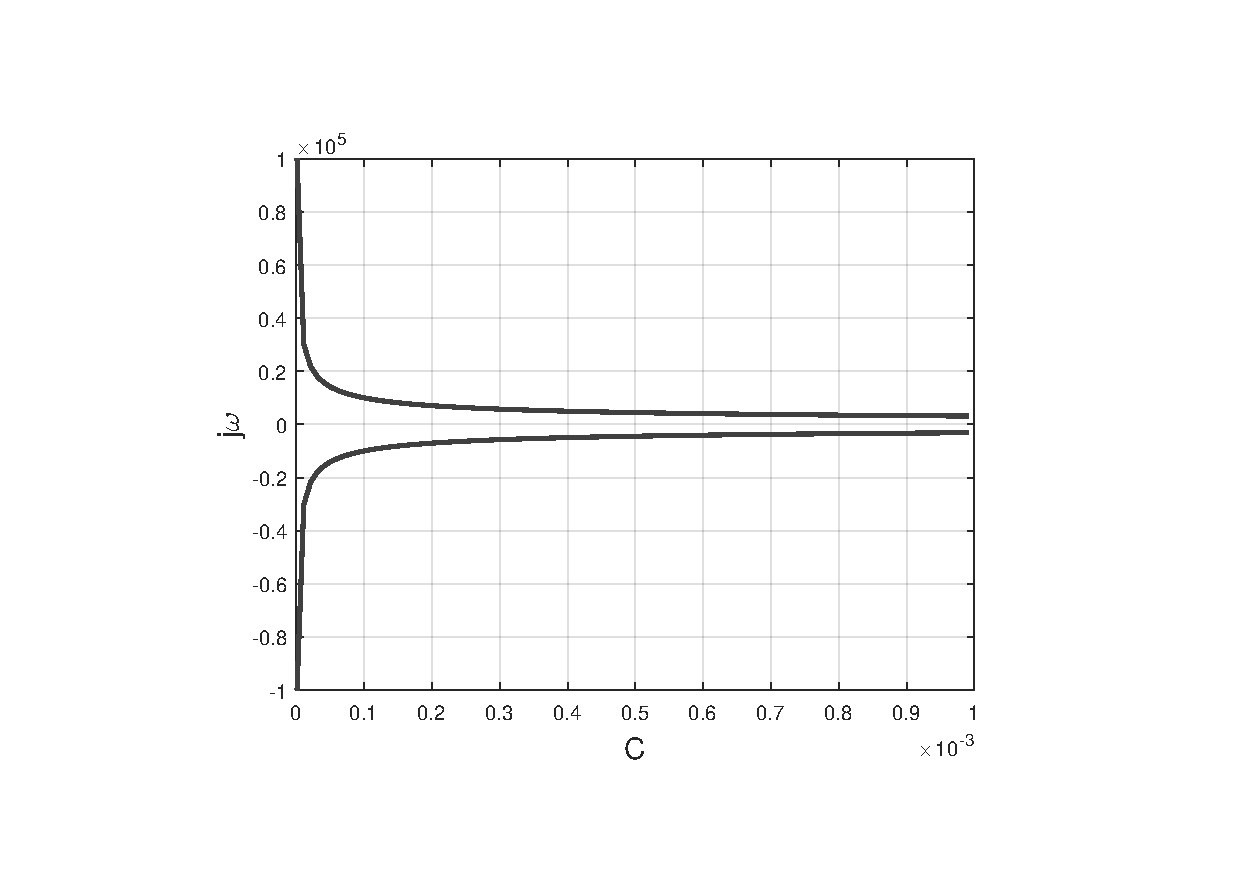
\includegraphics[width=\linewidth]{pd_imag_vs_c2}
			\caption{$j\omega$ vs $C_2$}
			\label{fig:pd_imag_vs_c2}
		\end{subfigure}
		\caption{Voltage source pole locus}
	\end{subfigure}
	\end{figure}
	Figure \ref{fig:pd_real_vs_l2}, figure \ref{fig:pd_real_vs_l2}, figure \ref{fig:pd_real_vs_c2}, and figure \ref{fig:pd_imag_vs_c2} depict the behavior of poles of the voltage source as the values of inductor and capacitor are changed. These plots are evident that the capacitor has no effect on the real part of the poles whereas the inductor influences bot the real and imaginary parts of the voltage source poles. As the capacitance increases, the imaginary part of the poles decreases nearly exponentially. This means that, increasing the capacitor value will reduce the oscillations, and hence improve the response to the disturbances.
	
	As the value of inductor is increased, the real part of the poles increases while the imaginary part of the poles decreases.  However, it is worth noting that the value of real part of the poles is always negative, so the converter is inherently stable. This implies that the value of inductor is a trade-off between the real and imaginary part of the poles. In other words, if the value of inductor is increased the response should become slower but the magnitude of oscillations due to disturbance would also decrease.
	\begin{figure}[h]
		\centering
		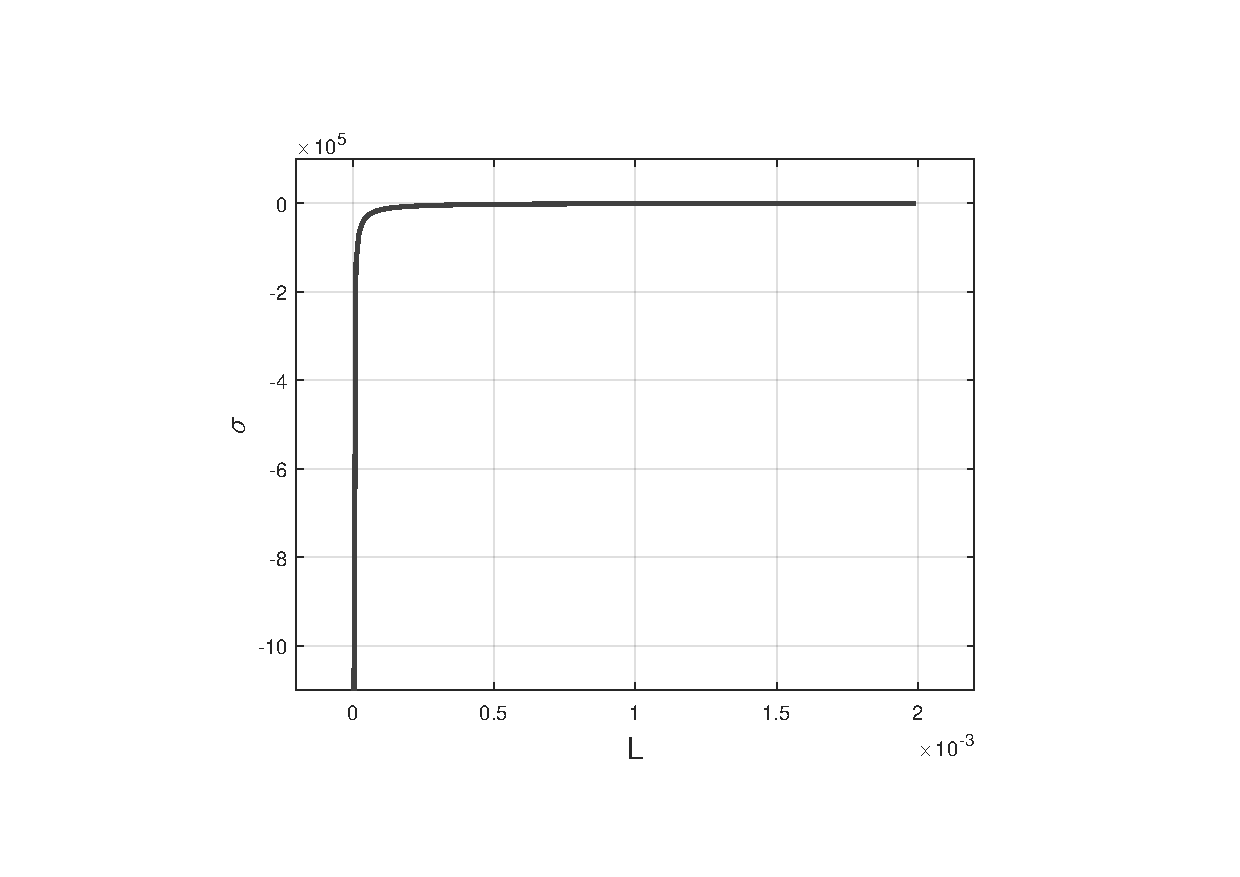
\includegraphics[width=0.6\linewidth]{pd_cs_l1}
		\caption{Current source pole locus: $\sigma$ vs $L_1$}
		\label{fig:pd_cs_l1}
	\end{figure}
	Figure \ref{fig:pd_cs_l1} shows the variation of the only pole of the current source with the value of inductor. As the value of inductor is decreased the response time of the current source decreases while the ripple increases. This fact is particularly useful in pulsed reference scheme discussed in chapter \ref{chap:lincontrol}. The current source must have a low enough rise time to respond to the pulsating reference. This has been verified via simulations.
	
	Based on the above discussion an inductor of 100 $\mu$H has been selected for current source and that of 2 mH for the voltage source during the practical implementation. A 1000 $\mu$F has been selected for the voltage source.	

\subsection{Snubber Design}
	Snubber is required across the ignition switch $Q_d$ to limit the over-voltage arising due to opening of the switch. In highly inductive circuits, when switch is opened, the path for current flow is broken. Therefore, a high voltage spike appears on the switch terminals due to large magnitude of $L\dfrac{di}{dt}$. Energy absorbing circuit like the snubber circuit, reduces these spikes. This section explains the design procedure for a R-C snubber used in parallel with the ignition switch $Q_d$.

	The peak current through the snubber circuit is given by
	\begin{equation}
		I_p = \dfrac{V_{oc}}{R_s}
		\label{eq:snub-1}
	\end{equation}
	where $V_{OC}$ is the open circuit voltage across the switch, $R_s$ is the snubber resistance and $I_p$ is the peak current through the snubber.

	The current flowing through $Q_d$ before interruption is $I_{\text{ref}}$ and the maximum voltage across the terminals of $Q_d$ is $V_{\text{ref}}$. Hence, the snubber resistance $R_s$ should be minimum of
	\begin{equation}
		R_s \geq \dfrac{V_{\text{ref}}}{I_{\text{ref}}}
		\label{eq:snub-2}
	\end{equation}
	The snubber capacitance should be such that:
	\begin{enumerate}
		\item Energy that is allowed to be stored in the capacitor should be greater than the energy stored in the inductor i.e.
			\begin{align}
				\dfrac{1}{2}C_sV_{oc}^2 &\geq \dfrac{1}{2}L_{eq}I_p^2\\
				\therefore C_s &\geq \dfrac{L_{eq}I_p^2}{V_{oc}^2}
				\label{eq:snub-3}
			\end{align}
		\item The snubber time constant must not exceed the minimum ON time of $Q_d$. So, for time constant of snubber circuit to be 10\% of the on time of $Q_d$
			\begin{align}
				R_sC_s &\leq \dfrac{T_{on}}{10}\\
				\therefore C_s &\leq \dfrac{T_{on}}{10R_s}
				\label{eq:snub-4}
			\end{align}
	\end{enumerate}
	From equations \eqref{eq:snub-2}, \eqref{eq:snub-3}, and \eqref{eq:snub-4}, $R_s$ is chosen $8 \Omega$ and $C_s$ is chosen as 2 $\mu F$

\section{Sensor Circuits and Calibration}
	A voltage and a current sensing is required for the normal operation of the proposed EDM power supply. However, an extra current sensor is required at the voltage source inductor if current mode control is to be utilised. Hence, a sensor board has been designed with three current sensors and two voltage sensors to acquire the required input variables for the controllers. These also account for sensing the load voltage and current through the spark gap. This section describes the individual components of this sensing board. 
\subsection{Voltage Sensors}
    \begin{figure}[h]
        \centering
        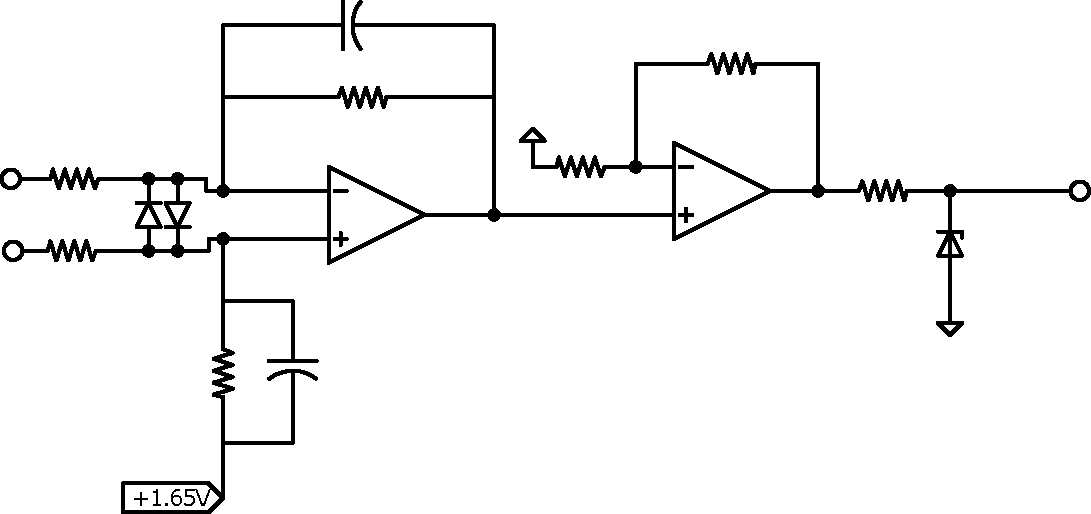
\includegraphics[width=0.8\linewidth]{voltage-sensor}
        \caption{Voltage sensing circuit}
        \label{fig:vsens}
    \end{figure}
	The voltage is sensed using potential dividers. Figure \ref{fig:vsens} shows the voltage sensing circuit. Two such circuits are required in the converter to measure the output voltage and the voltage source voltage. A differential amplifier with pre-tuned gain is used to measure the voltage. The output of differential amplifier is passed through a unity follower before reading by the ADC to overcome any current requirement shortcoming of the previous stage. It is worth noting that the operational amplifiers used in this hardware have a unity gain bandwidth if 3 MHz. A zener diode is used at the output for over voltage protection of the ADC. A reference voltage is manually added to extend the full scale measurement to negative voltages as the ADC is capable of measuring only positive voltages. The overall range of measurement is -120 to +130 V.
	\begin{figure}[h]
        \centering
        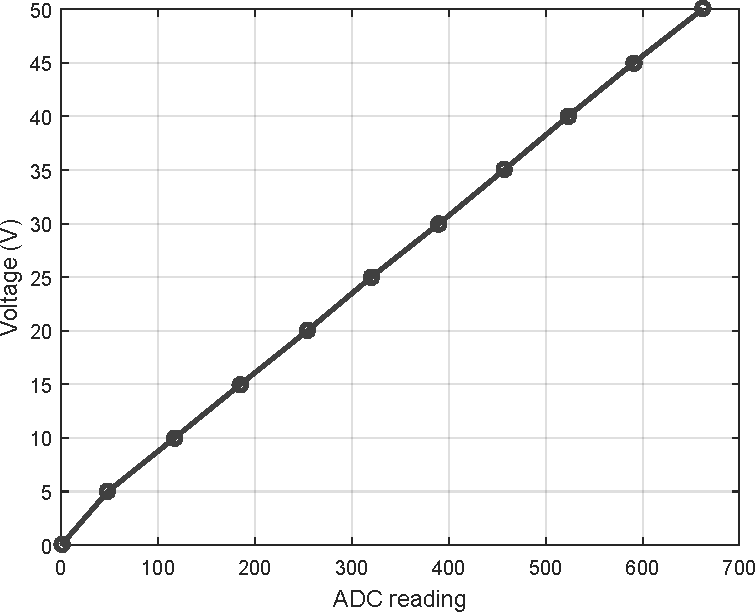
\includegraphics[width=0.6\linewidth]{voltage2_cal}
        \caption{Voltage sensor calibration}
        \label{fig:voltage2-cal}
    \end{figure}
	The calibration of the voltage sensor has been carried out by observing the ADC values as read by the DSP while the input voltage is varied from 0 to 50V in steps of 5V. A linearly regressed line is fitted through these points and the values of slope and the intercept are then used to calculate the actual voltage from the ADC values. Figure \ref{fig:voltage2-cal} shows the calibration curve for the voltage sensors. The Y-axis represents the voltage and X-axis represents the ADC readings.
	
	A hardware RC filter and a software averaging filter is required in this application due to very small gain requirements because of the large sensing ranges.
	
\subsection{Current Sensors}
    Various off-the-shelf current sensors have been tested for range, output voltage and frequency response before designing a shunt resistor based current sensing  circuits. Each sensor is tested for range by varying the amplitude of a square wave current signal. For testing the response time, the frequency of this signal is gradually increased till the rise time is about $1/5^\text{th}$ of the time period. Table \ref{tab:current-sensor} summarises the observations of these experiments.
	\begin{table}[h]
	\centering
		\begin{tabular}{| l | p{3cm} | p{4cm} | p{4cm} |} \hline
			\textbf{Sensor} & \textbf{Rating} & \textbf{Observations} & \textbf{Comments}\\ \hline
			HLSR 16P & \parbox[t]{3cm}{Voltage = 5V \\ Current = $\pm$40A \\ BW = 400kHz \vspace{1.5mm}} & Low sensed voltage & \parbox[t]{4cm}{$\text{Range}_\text{req}\ll\text{Range}_\text{rated}$ \\ Distortion above 20kHz} \\ \hline
			LA 55P & \parbox[t]{3cm}{Voltage = $\pm$15V \\ Current = $\pm$50A\\BW = 200kHz \vspace{1.5mm}} & Low sensed voltage & \parbox[t]{4cm}{$\text{Range}_\text{req} \ll \text{Range}_\text{rated}$ \\ Distortion above 10kHz} \\ \hline
			ACS 712 & \parbox[t]{3cm}{Voltage = 8V \\ Current = 100A\\BW = 80kHz \vspace{1.5mm}} & High rise time & Low bandwidth \\ \hline
			Shunt resistance & \parbox[t]{3cm}{Voltage = $\pm$5V \\ Current = $\pm$30A\\BW = 3MHz \vspace{1.5mm}} & Low rise time & \parbox[t]{4cm}{Adjustable gain and BW} \\ \hline
		\end{tabular}
		\caption{Current sensor testing}
		\label{tab:current-sensor}
	\end{table}
    \begin{figure}[h]
        \centering
        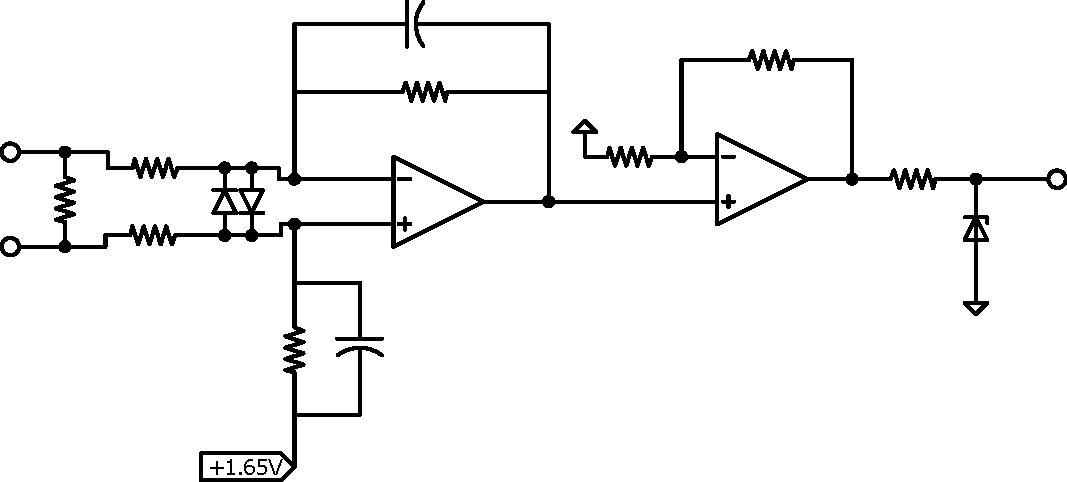
\includegraphics[width=0.8\linewidth]{current-sensor}
        \caption{Current sensing circuit}
        \label{fig:isens}
    \end{figure}
    The voltage drop across a shunt resistor of 0.1 $\Omega$ and 20 W is used to measure the current. Figure \ref{fig:isens} shows the current measurement circuit. The voltage across shunt resistor is fed to differential amplifier circuit to increase the gain. This is then fed to a unity follower. The output protection and bias arrangements are same as the voltage sensor. Three such circuits are required to measure the currents in both inductors and the load current The range of current measurement achieved is -15 to +20 A.
	\begin{figure}[h]
        \centering
        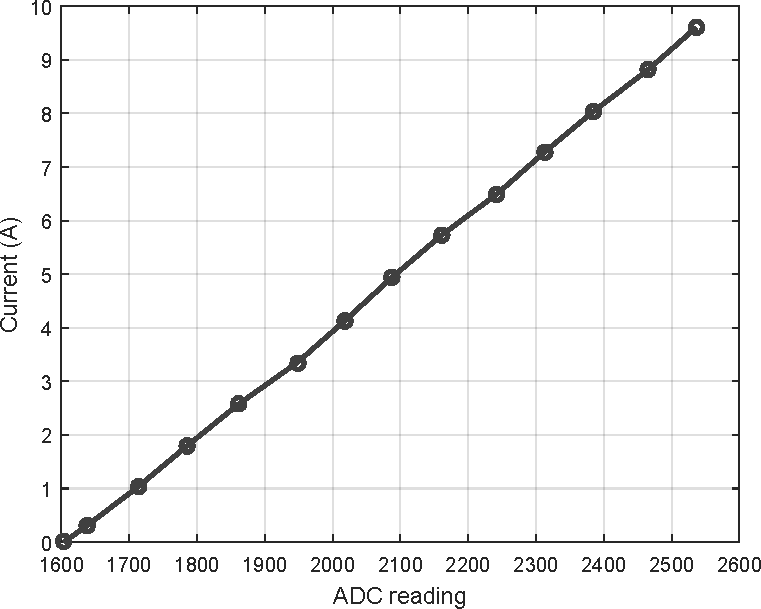
\includegraphics[width=0.6\linewidth]{current2_cal}
        \caption{Current sensor calibration}
        \label{fig:current-cal}
    \end{figure}
	The calibration of current sensor has been carried out via the same procedure as the voltage sensor. The current is varied from 0 to 10A in small steps, then a linear regression curve is fitted through this data. The values of slope and the intercept are then used to obtain the current reading from the ADC values. Figure \ref{fig:current-cal} shows the calibration curve for the current sensor. The Y-axis represents the current values while the X-axis represents the ADC values. No filtering is employed in the current sensor to preserve the small response times.

\section{Power Electronic Switches}
	Initially, every part of the hardware was designed and components were chosen from electronic components available in the market. The details of this MOSFET-based design are given in appendix \ref{app:mosfet-based}. However, considering time constraint and reliability of operation, the power electronic switches along with driver are sourced as ready to use IGBT modules/stacks from Semikron. Following section describe these in brief.
	\begin{figure}[h]
        \centering
        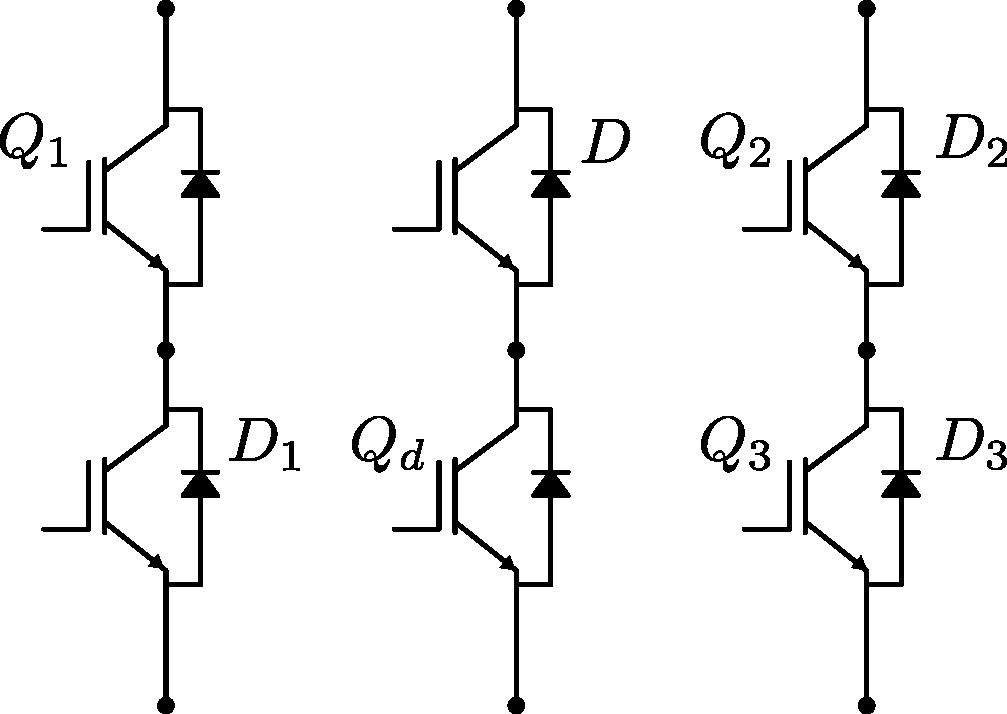
\includegraphics[width=0.4\textwidth]{igbt}
        \caption{IGBT module configuration}
        \label{fig:igbt}
    \end{figure}
    Figure \ref{fig:igbt} is representation of the IGBT modules used for switching in the proposed converter topology. The first module is used as the current controlled single quadrant converter with devices $Q_1$ and $D_1$ as marked. The switches $Q_2$ and $Q_3$ from the last module are acting as voltage controlled two quadrant converter. The ignition control scheme is realised using the second module with devices $Q_d$ and $D$. The diodes $D_1$ and $D$ are the body diodes of the IGBTs which always remain OFF during the entire operation. The rating of the switches in the ignition control module is 1200 V, 88 A, 20 kHz while that of the two converter modules is 600 V, 150 A, 500 kHz.
	\begin{table}[h]
		\centering
		\begin{tabular}{| l | l | p{4cm} |} \hline
			\textbf{Module} & \textbf{IGBT} & \textbf{Rating} \\ \hline
			1, 3 & SKM145GB066D & \parbox[t]{4cm}{$V_{CE}$=600V \\ $I_{C}$=190A \\ $I_D$=150A \\ $t_r$=52ns \\ $t_f$=45ns \\ $t_{d(ON)}$=150ns \\ $t_{d(OFF)}$=450ns} \vspace{-1mm} \\ \hline
			2 & SKM75GB12T4 & \parbox[t]{4cm}{$V_{CE}$=1200V \\ $I_{C}$=115A \\ $I_D$=97A \\ $t_r$=39ns \\ $t_f$=66ns \\ $t_{d(ON)}$=150ns \\ $t_{d(OFF)}$=370ns} \vspace{-1mm} \\ \hline
		\end{tabular}
		\caption{IGBT module ratings}
		\label{tab:igbt}
	\end{table}

	\section{DSP Board}
	\begin{table}[h]
	\begin{tabular}{|l|l|l|l|} \hline
	\textbf{Function} & \textbf{Number of units} & \textbf{Rating} & \textbf{Utility} \\ \hline
	CPU & 1 & 90 MIPS & Executing control laws \\ \hline
	CLA & 1 & 90 MIPS & Sampling and filtering ADC inputs \\ \hline
	ADC & 16 & 0 to 3.3 V, 3.46 MSPS & 5 channels for sensing\\ \hline
	ePWM & 16 & $\text{V}_\text{L}$ = 0V, $\text{V}_\text{L}$ = 3.3 V & 6 channels for IGBTs\\ \hline
	\end{tabular}
	\caption{DSP specifications}
	\label{tab:dsp}
	\end{table}
	
    The F28069 Piccolo series processor operates at 90 MHz system clock. Table \ref{tab:dsp} summarises the important specifications of this DSP. Six ePWM channels and five ADC channels from this processor are utilised in the normal operation of the pulsed power supply. The ADC sampling and controller execution frequencies are set to 50 kHz.

    Figure \ref{fig:interfacing} shows the interfacing circuit for switching signals from the ePWM channel output to the gate driver input of the IGBT modules. A voltage buffer is used to change the voltage level of switching signals from 3.3 V to 15 V as per the requirements of the gate driver circuit. A unity follower is used to mitigate voltage drop issues due to the current requirements of the gate driver.

	\begin{figure}[h]
        \centering
        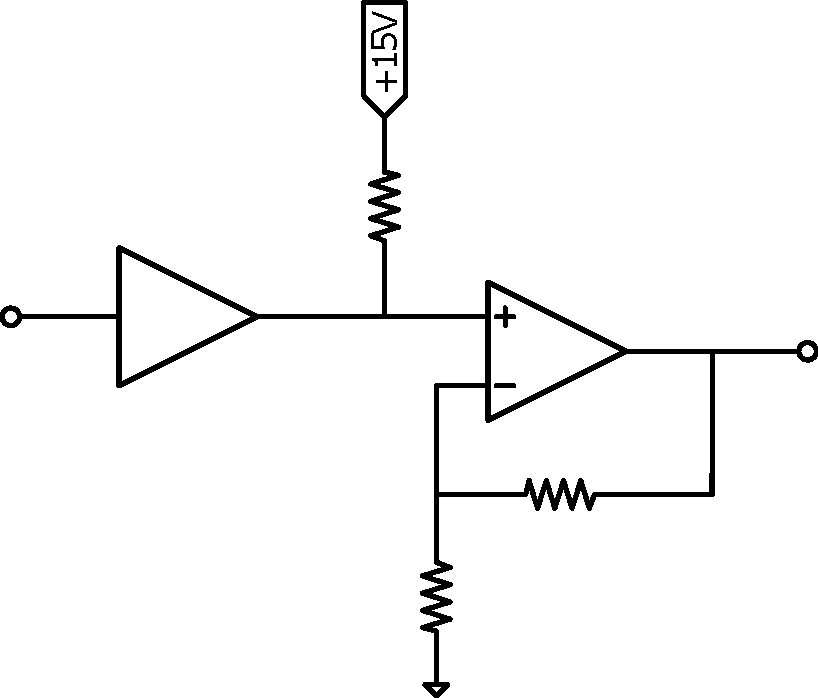
\includegraphics[width=0.4\textwidth]{interfacing}
        \caption{DSP interfacing circuit}
        \label{fig:interfacing}
    \end{figure}
	\begin{figure}[h]
        \centering
        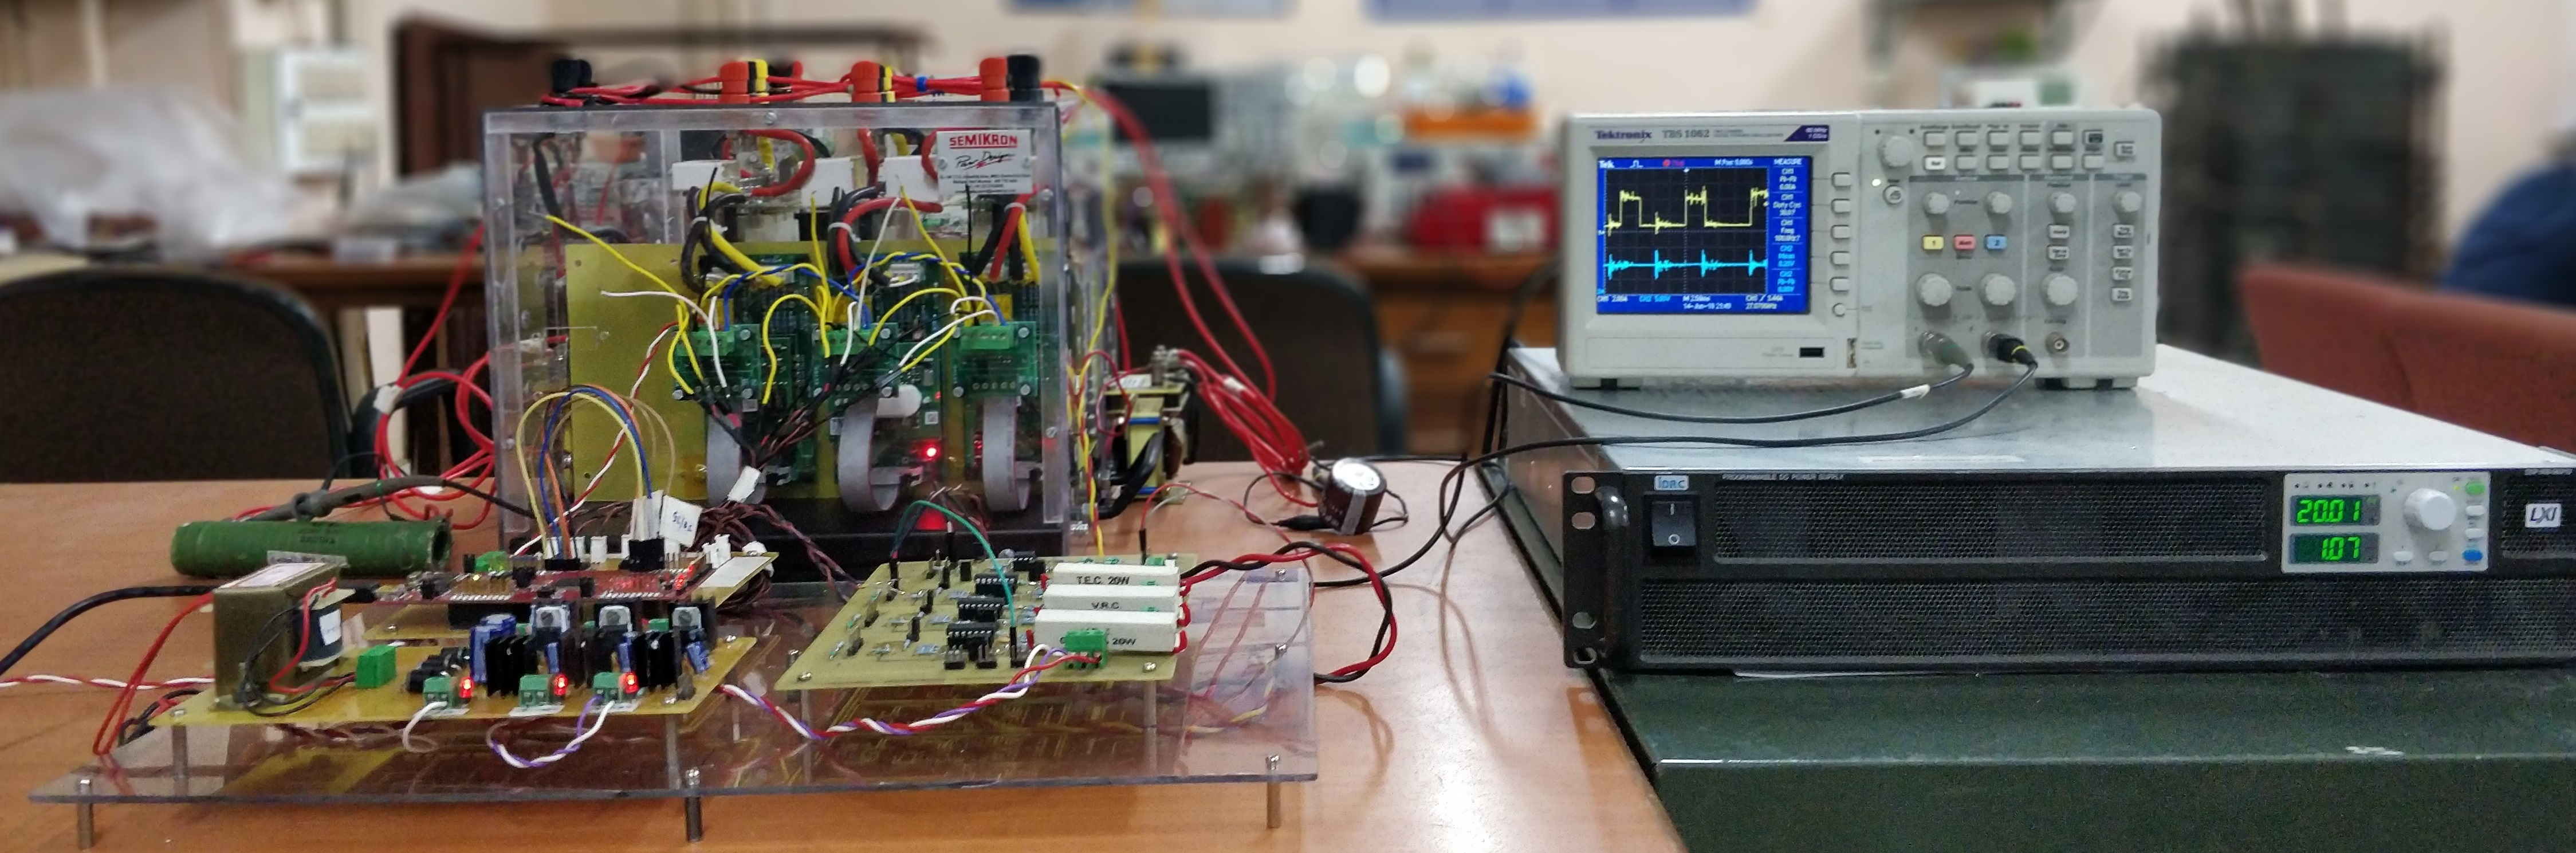
\includegraphics[width=0.8\textwidth]{setup}
        \caption{Complete experimental setup of pulsed power supply}
        \label{fig:setup}
    \end{figure}
    \begin{figure}[h]
        \centering
        \includegraphics[width=0.7\textwidth,angle=90]{interfacing-image}
        \caption{DSP interfacing hardware}
        \label{fig:interfacing-image}
    \end{figure}
